        The intermediate code list ({\bf TDE list})is not a linked netlist in
        the usual sense. In a conventional netlist each net is a single signal
        linked to one or more logic element inputs and a single element output
        (unless a 3-state output). The intermediate code list employs TDEVar
        class instances to represent signals.

        The TDEVar class represents a signal or signals in the intermediate
        code. A TDEVar may have an associated WordSpec which describes the
        signals in an array or struct, the type(s) these represent and
        optionally the variable for which the TDEVar was created.

        In the simplest case a TDEVar may represent a logical signal controlling
        the flow of execution. For example an execution thread is just a logical
        high passed along a chain of delay or control elements. Conditional
        control signals also enable static variable assignments, memory reads
        and writes and queue pushes and pops. These simple single signals in
        most cases do not have an associated WordSpec, or if they do it has
        primitive type LOG. These TDEVars usually have compiler generated
        identifiers such as "S123" (these cannot clash with identifiers from 3PL
        source code variables).

        TDEVars also represent inputs or outputs of variables or expressions
        (including constants). In that case they have an associated WordSpec
        which indicates the primitive types and bits of a variable and its
        fields or array members.

        A TDEVar representing a value, for example the output of a static
        variable, is created when the need arises in generating logic during
        immediate execution. If multiple distinct instances of the same value
        are created this does not affect the conversion of intermediate code
        into the EDIF netlist as netlist names are generated from the identifier
        and the specified bits of the variable. Thus separate insances of the
        same TDEVar come together as connected when converted to the netlist
        since they share the same identifier and bit specification, i.e. they
        are imlicitly rather than explicitly connected. Even though this scheme
        is logically correct it does pose problems for optimisation as it is not
        possible within the intermediate code to recognise that identical TDEVar
        instances represent the same signals and will indeed lead ultimately to
        shared netlists. As a means of obviating this problem a map of created
        TDEVars is kept. Each TDEVar is entered into the map (catalog) with the
        identifier as key. The entries under each key are lists of instances of
        TDEVars. When a TDEVar instance is to be created the list from the map
        entry for that identifier is searched for an identical bit specification
        (provided by the WordSpec). If one is found then that TDEVar is
        returned, otherwise a new one is created and entered into the map. This
        avoids duplication of TDEVars and means that separate references to the
        same value are via a common TDEVar which implies that they are connected
        in the intermediate code list. Thus optimisation code can locate all
        sources and sinks for a value and effect any useful optimisation.

        The TDEVar catalog is not applied universally. In many cases the TDEVars
        carry additional information in the associated WordSpec which varies from
        instance to instance, for example variable subscripts. But since the
        logic is still correct even when TDEVar duplication cannot be avoided
        these exceptions do not invalidate the process.

        TDEVars may be explicitly connected in the TDE list by two
        means -
        \blist
        \item   a CONNECT TDE
        \item   method TDEVar.merge()
        \blend
        In both cases the identifiers will be different as otherwise TDEVars are
        implicitly connected as explained above and do not need explicit
        connection.

        A CONNECT TDE explicitly connects two TDEVars. The CONNECT TDE is also
        able to expand or truncate connections between input and output where
        the signals are of different size.
        
        The merge() method is only called in method TDEList.optimise() and is
        restricted to the following specific situations -
        \blist
        \item   merging of TDEVars which specify complete variables, i.e.
                the associated WordSpecs will have the {\bf complete}
                field true, and which have the same number of bits.
        \item   merging of single control signals
        \item   merging of clock signals
        \blend


        \subsection{TDEVar fields}


        
            {\bf String id}
            
            The variable identifier if {\bf TDEVtype.VAR} (actually if it is
            not type {\bf TDEVtype.VAR} it will have an identifier similar
            to "CONST123" but this is solely for diagnostic labelling purposes
            and is not used by the compiler).

            {\bf TDEVtype type}
            
            This distinguishes between a normal TDEVar, {\bf TDEVtype.VAR}, and
            a constant. When a TDEVar is a constant it is an implicit signal
            array source. The type of constant is given by this field with
            values {\bf TDEVtype.BITS}, {\bf TDEVtype.UINT}, {\bf TDEVtype.INT}
            and {\bf TDEVtype.BOOL}. The actual value of the constant is stored
            in field {\bf Object val}. A constant TDEVar is converted to a
            signal array, sourced with a pattern of connections to VCC and GND
            representing the value, during netlist structure generation.

            {\bf WordSpec wordspec}
            
            If this TDEVar is a value array then this field describes the
            word boundaries and the word types of this reference.
            
            If this TDEVar is an execution signal then this field is null.

            {\bf Object val}
            
            Value if a constant - see {\bf TDEVtype type} above. Otherwise
            this field is null.
            
            {\bf SrcLoc loc}
            
            Source file location where this TDEVar was generated.

            {\bf Common common}
            
            The {\bf Common} subclass is described in the following section. It
            is used to link connected TDEVars which are simple control signals,
            clock signals or represent complete variables (not array members or
            struct fields).
            
            {\bf private static HashMap\verb'<'String,ArrayList\verb'<'TDEVar\verb'>>' catalog}
            
            This static variable maps signal identifiers to all TDEVars which
            have that identifier.
 
            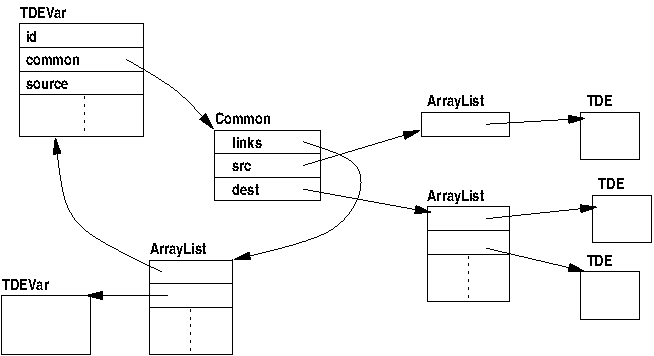
\includegraphics{TDEVar}




        \subsection{Common class}
        
            Every TDEVar contains a {\bf common} field. Where two TDEVar
            instances represent the same signal or signal array they can be
            merged by combining their common fields into a single shared
            object.
            
            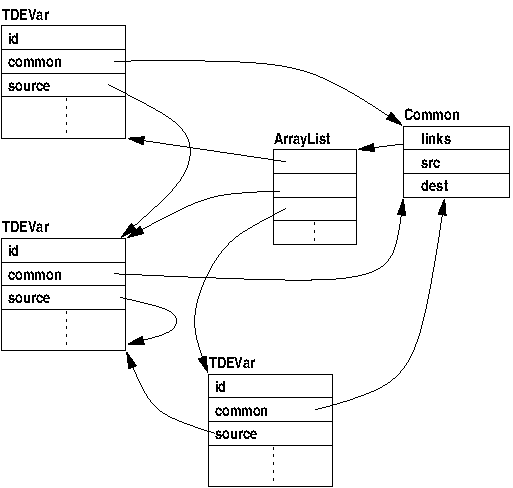
\includegraphics{TDEVarCommon}            
                      
            For example in the following 3PL code -
            
            \begin{lstlisting}[gobble=12, language=threepl]
                static(global.s1, "uint:4");
                static(global.s2, "uint:4");
                .
                .
                s1 <- s2;
                .
                .
            \end{lstlisting}
            
            The LHS reference in line 5 will generate a TDEVar which will appear
            in the TDE list as {\bf glob.s1.D[0..3]}, i.e. the D or data input
            to register s1. The RHS expression in line 5 will contain a TDEVar
            listed as {\bf glob.s2[0..3]}, the output of register s2.
            
            The assignment statement will connect the s1 data input to the
            s2 output, the s1 CE input (clock enable) to a control signal that goes high
            when the statement is executed and the s1 RES (reset) to GND.
            
            \begin{lstlisting}[gobble=12, language=tde]
            .
            .
            FMOD1/glob.s1.D[0..3] = FMOD1/glob.s2[0..3]
            FMOD1/glob.s1.CE[0..3] = S123
            FMOD1/glob.s1.RES[0..3] = GND
            .
            .
            REG
	            OUT  FMOD1/glob.s1[0..3]
	            <-
	            CLK  glob.c166
	            D    FMOD1/glob.s1.D[0..3]
	            CE   FMOD1/glob.s1.CE[0..3]
	            R    FMOD1/glob.s1.RES[0..3]
                {0x0}
            \end{lstlisting}
            
            After optimisation the CONNECT TDEs will be removed and the merged
            TDEVars will result in -
            
            \begin{lstlisting}[gobble=12, language=tde]
            .
            .
            REG
	            OUT  FMOD1/glob.s1[0..3]
	                        <-
	            CLK  glob.c166
	            D    FMOD1/glob.s2[0..3]
	            CE   s123
	            R    GND
                {0x0}
            \end{lstlisting}
            
            The funtionality has not changed and the merges are not logically
            necessary, but the TDE list is shorter and easier to read.

            The fields in common are -
            \blist
            \item   {\bf Clock clock\_var} \\
                    This is the clock variable for the clock domain of the
                    TDEVar(s). Constant TDEVars do not have a clock domain in
                    which case this is null.
            \item   {\bf ArrayList\verb'<'TDE\verb'>' dest} \\
                    A list of TDEs which are destinations (sinks) for this signal.
            \item   {\bf ArrayList\verb'<'TDE\verb'>' src} \\
                    A list of TDEs which are sources for this signal.
            \item   {\bf ArrayList\verb'<'TDEVar\verb'>' links} \\
                    TDEVars whose sources point here
            \blend

        
        \subsection{the merge method}
        
            As immediate execution proceeds connection of signals is done by
            method TDEList.connect(). This generates a {\bf CONNECT} TDE with one
            input TDEVar (the source) and one output TDEVar (the destination). If
            the input and output are different sizes then this represents a cast()
            which will pad or truncate the input array to match the output array.
            The input may even be a single signal to be connected to each bit of
            an output array, often the case with input GND or VCC.

            These CONNECT TDEs are resolved when processed by
            netlist.Xilinx.XTDECode(), however the presence of these CONNECT TDEs
            makes the intermediate netlist code difficult to read. As a dump of
            the intermediate netlist is a useful resource for checking the
            generated code for validity or determining problems with combinatorial
            expressions failing timing constraints, some effort has gone into
            resolving some of these {\bf CONNECT} TDEs during optimisation of the
            intermediate netlist, thus simplifying the presentation substantially.
            Note that this simplification is not required for generation of the
            final EDIF file from the intermediate netlist, it is simply to improve
            readability.

            The process is carried out during optimisation by examining all {\bf
            CONNECT} TDEs (there is a list of them in class TDEList) and where
            appropriate merging the set of destination TDEVars with the source
            TDEVar. This is done by method TDEVar.merge() using the common class.
        
            Method {\bf merge()} is called to merge two TDEVars. Before
            calling this method it must be determined that the two TDEVars
            meet one of the following criteria - 
            \blist
            \item  the TDEVars are for control signals (WordSpec is null).
            \item  the TDEVars are for clocks signals.
            \item  the TDEVars are for complete variables.
            \blend          
            This method does not perform these checks itself.
            
            The TDEVar to which merge() is applied should be the source and the
            argument to merge() should be a destination (sink). The source ID
            is used as the preferred ID.

            \begin{lstlisting}[gobble=8, language=java, xleftmargin=1cm]
            public void merge (TDEVar dtdev) {
                Common  dc = dtdev.common;   // destination common
                Common  sc = common;         // source common
                String  old_dest_id = dtdev.id;
                String  sid = id;

                sc.src.addAll(dc.src);                  // add source TDEs
                sc.dest.addAll(dc.dest);                // add destination TDEs
                sc.links.addAll(dc.links);              // link destination TDEVar links to the source of this TDEVar

                for (TDEVar t : dc.links) {
                    t.id = sid;
                    t.type = type;
                    t.wordspec = wordspec;
                    t.common = sc;
                    t.val = val;
                }

                // Update all occurrences of destination TDEVars with the same id
                // with the new source id.
                ArrayList<TDEVar>   al = catalog.get(old_dest_id);
                for (TDEVar tdev : al) {
                    if (tdev == dtdev)
                        continue;
                    tdev.id = sid;
                }
            }
            \end{lstlisting}

            Both the source TDEVar (this) and destination TDEVar (dtdev) may already
            have other TDEVars linked via their respective Commons as a result of
            previous merges. As a minimum every TDEVar has a link to itself in its
            Common.

            The destination common src, dest and links lists are appended to the
            corresponding lists in the source common.

            The source TDEVar will already have the same ID, type, WordSpec, Common
            class instance and val field in all linked TDEVars as result of previous
            merges. All linked destination TDEVars now have the source ID, type,
            WordSpec, Common and val field written into them. The merged destination
            TDEVar will now have the same ID, type, WordSpec, Common and val fields
            as the source TDEVar.

            Now that the destination TDEVars have had their IDs changed, any other
            instances of a TDEVar with the same ID, regardless of linkages or
            WordSpec, must be have their IDs changed as well. This is done using the
            catalog map.

            


        \subsection{target variables}

            Program target variables may be global, in which case the associated
            signal names begin with "glob.". Thus the output of a static global
            variable {\em a} would be a signal named {\em glob.a}.
            
            All other target variables are prefixed by a string constructed from all
            the hierachical scopes within which they are created. Each scope has an
            associated identifier which is either a module, procedure or function
            identifier or else a control structure indicator such as "if" or "when".
            Unique integers are appended to these identifiers to avoid duplication
            that might result from repeated entry to a scope. A target variable {\em
            b} created within a source file prog.3pl would have the identifier {\em
            prog.b}. If it was created after calling procedure proc then it would be
            {\em prog.proc\_1.b}. If the procedure were called again the resulting
            variable would be {\em prog.proc\_2.b}. A variable {\em c} created
            within a 'for' loop would have identifiers {\em prog.proc\_1.for\_1.c},
            {\em prog.proc\_1.for\_2.c} etc.
            
            Hierarchical signal names must include file paths of source files. To
            avoid very long identifiers file paths from {\bf source} or {\bf module}
            statements are replaced by arbitrary strings SRCn or FMODn in
            identifiers, {\bf n} being an integer. The optional intermediate code
            report file (prog.icl) lists these for reference purposes.

            Signal array references have a subscript range appended, even
            if the entire variable is accessed, e.g. "glob.a[0..7]". For
            multiple ranges comma-separated ranges are shown, e.g.
            "glob.a[0..7,16..23]"

            \subsubsection{static variables}

                A global static variable {\em s} of size 8 bits would have
                the following associated signal arrays -
                \blist
                \item   "glob.s[8]" - the data output signal array
                \item   "glob.s.D[8]" - the data input signal array
                \item   "glob.s.CE[8]" - the clock enable signal array
                \item   "glob.s.RES[8]" - the reset signal array
                \blend                
                The value of the variable is available via the data output
                signal. Assignments are made by driving the data input
                signal and asserting the clock enable signals to the selected
                bits. The reset signal array is used to return some
                portion of the variable to its initial state.

            \subsubsection{queue variables}

                A global queue variable {\em p} of size 8 bits would have
                the following associated signal arrays -
                \blist
                \item   "glob.p[8]" - the data output signal array
                \item   "glob.p.D[8]" - the data input signal array
                \item   "glob.p.NE" - output availability (not empty)
                \item   "glob.p.POP" - pop a datum
                \item   "glob.p.PUSH" - push a datum
                \item   "glob.p.NF" - input availability (not full)
                \item   "glob.p.CNT[4]" - buffer occupancy count
                \item   "glob.p.SPC[4]" - buffer space count
                \item   "glob.p.RSTAT[5]" - buffer status in read clock domain
                \item   "glob.p.WSTAT[5]" - buffer status in write clock domain
                \blend
                These signals are further described in the section on queue
                buffers below.

            \subsubsection{value variables}

                Value variables are effectively pointers and can be
                assigned multiple times. To ensure that each assigned
                value is distinguished a unique integer is appended.
                A global value variable {\em v} of 8 bits might thus appear
                variously as "glob.v\_1", "glob.v\_2" etc.                
                At the
                completion of immediate program execution the signal array
                "glob.v" would be equated with the last value the variable was
                assigned. This is an attempt to give the unappended variable
                identifier a sensible value during simulation.

            \subsubsection{priority variables}

                A global priority variable {\em p} of size 8 bits would have
                the following associated signal arrays -
                \blist
                \item   "glob.p[8]" - the data output signal array
                \item   "glob.p.D[8]" - the data input signal array
                \item   "glob.p.PE" - the 'else' signal
                \blend


            \subsubsection{memory variables}

                Memory variables have separate signal array identifiers
                for each port, e.g. global combinatorial-output memory
                {\em m} with two ports would have port output signal arrays
                "glob.m\_0" and "glob.m\_1".


        \subsection{expressions and execution control signals}

            The values resulting from expressions are given signal array
            identifiers of the form "E9".

            "startex" is a level signal which is asserted to begin
            execution. It is resynchronised to every clock domain, for example
            for a global clock {\em clk} the resynchronised start signal
            would be "glob.clk.start".

            Various other control signals are generated with prefices
            "A", "AND", "CD",, "CONST" "EO", "F", "FB", "FD", "FDCP", "FDRS",
            "FF", "FS", "I", "IN",, "INT" "INV", "LOG", "MADDR", "MDATA", "P",
            "PE", "PNTBUSY", "Q", "RADDR\_", "ROPAV", "S", "SAMPLEOUT", "SB",
            "SC", "SD", "SS", "start", "TF", "TS", "UINT" and "WADDR\_", integers
            being appended in each case to ensure identifiers are unique. there
            is no particular significance in these identifiers, the initial
            strings having been chosen to reflect the context in an attempt
            to improve readability of the intermediate code.

